\chapter{Testování a ověření správnosti}

% - hry pouze jako demonstracni a testovaci prvek
% - nestest, porovnani vystupu se vzorovym vystupem
% - instr_test-v5, vsechno je vyborny krome 2 neoficialnich instrukci (SHX a SHY pokud se nemylim),
%   ktere byly zavisly na sumu na sbernici.
% - vlastni unit testy CPU
% - vyuziti mesenu pro zkoumani chovani nes her a take je to vzorovy emulator
% - nas emulator je celkem presny za vyjimkou velice specifickych detailu, ktere jsou dusledkem
%   designu cipu a hardwaru nes

Testování probíhalo v několika úrovních -- od izolovaných unit testů procesoru a testovacích
programů až po porovnání s referenčními emulátory.

\section{Testování CPU}

Při implementaci emulátoru CPU byla vytvořena sada unit testů pomocí knihovny Unity. Tyto testy
sloužily jako prvotní ověření správnosti implementace a zaměřovaly se na funkčnost jednotlivých
instrukcí a jejich cyklovou přesnost.

Pro důkladnější testování byly využity veřejně dostupné testovací programy:

\begin{itemize}
    \item \textbf{Nestest} -- tento testovací program generuje log o stavu všech registrů a počtu
        uplynulých cyklů po každé vykonané instrukci. Výstup emulátoru byl automatizovaně
        porovnáván s referenčním logem (\textit{golden log}), což umožnilo přesně identifikovat
        případné odchylky v chování a časování CPU.
    \item \textbf{Blargg's}\footnote{Autorem je uživatel fóra NESDev s přezdívkou ,,Blargg'', který
        velice aktivně se věnoval zkoumaní architektury NES a návrhu testovacích programů pro
    emulátory.} \textbf{Instruction Tests (instr\_test-v5)} -- tato sada ROM souborů testuje
    pokročilé aspekty CPU, včetně neoficiálních instrukcí. Emulátor úspěšně prošel všemi testy s
    výjimkou neoficiálních instrukcí \texttt{SHA}, \texttt{SHX}, \texttt{SHY} a \texttt{TAS}. Tyto
    instrukce závisejí na aktuálním stavu a šumu na datové sběrnici, proto jejích emulace je celkem
    obtížná. Navíc tyto instrukce se téměř nepoužívají, proto absence jejich emulace neuškodí
    kompatibilitě emulátoru.
\end{itemize}

\section{Komplexní testování}

Na rozdíl od CPU, PPU a APU se netestovaly izolovaně pomocí unit testů, nýbrž prostřednictvím
porovnání s referenčním emulátorem \textbf{Mesen}, který je považovan za jeden z nepřesnějších
emulátoru NES\cite{mesen}, a předmětem testování byly komerční hry a testovací programy. Komerční
hry byly využité hlavně na testování PPU a na ověření, zda jednotlivé emulované komponenty
spolupracují správně.

Komerční hry také dovolovaly testovat správnost emulace APU, ale jelikož většina her nevyužívá
všechny možností APU, správnost se dalo ocenit jen hrubě. Pro detailnější testování byl využit
program \textbf{livenes}, který funguje jako syntezátor, kde uživatel může přepínat jednotlivé bity
registrů APU (obr. \ref{fig:livenes}). Díky tomuto programu bylo možné tence otestovat jednotlivé
aspekty APU.

\begin{figure}[H]
    \centering
    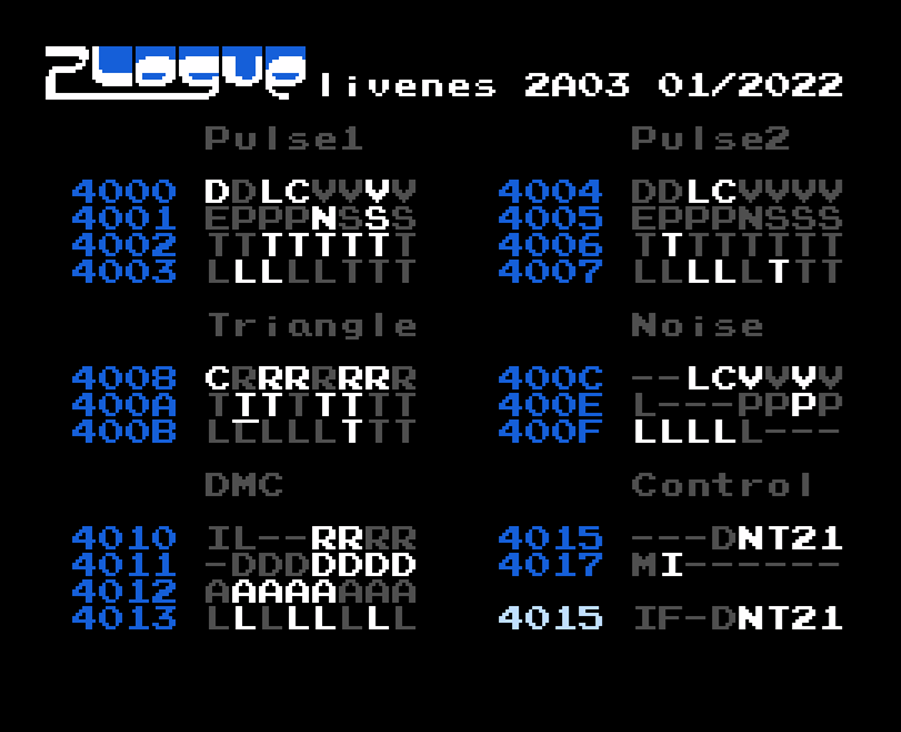
\includegraphics[width=0.5\textwidth]{images/livenes.png}
    \caption{Program livenes, který dovoluje přepínat jednotlivé bity registrů APU.}
    \label{fig:livenes}
\end{figure}

V případě PPU jedním z užitečných programů pro ověření správností grafického výstupu byl program
\textbf{240p-test-mini}. Tento program poskytuje rozsáhlou sadu testů pro ověření správností
grafického výstupu, přičemž nejen emulátoru, ale také monitoru nebo televizoru (obr. \ref{fig:240p-1}
a \ref{fig:240p-2}).

\begin{figure}[H]
    \centering
    \begin{subfigure}{0.45\textwidth}
        
\includegraphics[height=6cm]{images/240p-1.png}
        \caption{Test \textit{SMPTE color bars}.}
        \label{fig:240p-1}
    \end{subfigure}
    \quad
    \begin{subfigure}{0.45\textwidth}
        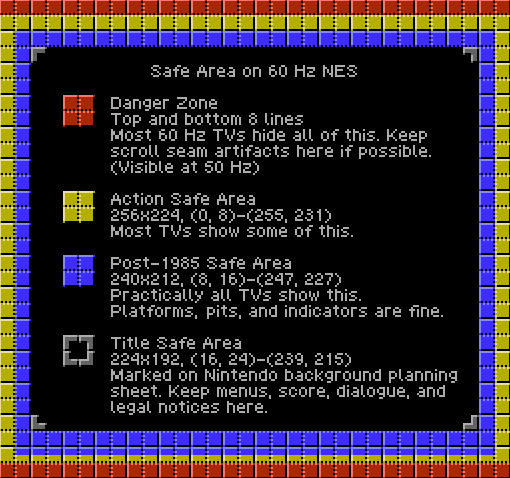
\includegraphics[height=6cm]{images/240p-2.png}
        \caption{Test \textit{Safe areas}.}
        \label{fig:240p-2}
    \end{subfigure}
    \caption{Testovací sada 240p-test-mini.}
    \label{fig:240p}
\end{figure}

% Pro tenčí testování a ověření správností na úrovní detailů a hardwarových quirku, se plánuje použit
% velké množství testovacích programů a stress testů obsažených v \cite{nesdev-emulator-tests}. Jsou
% tam obsazene programy, ktere testuji hardwarove quirky a detaily CPU, PPU a APU, ve kterych se casto
% implementace chybuje nebo jsou prehlizeny.

Pro hlubší verifikaci a ověření správnosti emulace na úrovni nejjemnějších detailů se v další fázi
vývoje plánuje nasazení rozsáhlé sady specializovaných programů a zátěžových testů obsažených v
archivu \cite{nesdev-emulator-tests}. Tyto testy jsou navrženy k odhalení specifických hardwarových
vlastností, které jsou pro platformu NES typické, avšak v softwarových
implementacích bývají často opomíjeny nebo chybně implementovány. Pozornost bude věnována zejména
kritickým aspektům časování instrukcí a reakce CPU na přerušení, komplexnímu chování PPU během
vykreslování a precizní syntéze v rámci APU.

\section{Benchmarking a profilování}

Základní metrika výkonu byla získána měřením času potřebného pro kompletní vygenerování jednoho
snímku. K tomuto účelu byly využity hardwarové časovače poskytované knihovnou Pico SDK,
přesněji funkce \texttt{time\_us\_32()} (výpis \ref{lst:frame_time}).

\begin{listing}[htbp]
\begin{minted}{c}
while (true) {
    unsigned t_start = time_us_32();

    update_joypads(&self->bus.joypad1, &self->bus.joypad2);
    disable_interrupts();

    if (self->reset_required) {
        /* ... */
    }

    enable_interrupts();
    bus_update(&self->bus);
    run_frame(self);

    unsigned t_end = time_us_32();
    /* Uložení rozdílu času před a po emulaci snímku */
    frame_times[frame_time_idx] = t_end - t_start;
    /* Výpis naměřených hodnot a jejích průměr */
    if (frame_time_count >= FRAME_TIMES_TOTAL) {
        frame_time_idx = 0;
        print_average_frame_time();
    }
}
\end{minted}
\caption{Měření průměrného času, potřebného na emulaci jednoho snímku.}
\label{lst:frame_time}
\end{listing}

% Hodnoty potřebného času pro vykreslení snímku se měřily v menu BIOS a v několika komerčních hrách,
% přitom se vybíralo se 10vzorků

% Měření probíhalo v hlavní emulační smyčce. Před zahájením emulace snímku byla zaznamenána počáteční
% hodnota časovače v mikrosekundách a po dokončení vykreslení snímku PPU (včetně neviditelných
% scanlinů) byla zaznamenána hodnota koncová. Rozdíl těchto hodnot představuje čistý výpočetní čas.
% Pro eliminaci ojedinělých výkyvů a získání statisticky relevantních dat byl implementován buffer o
% velikosti $N$ prvků. Do tohoto pole se průběžně ukládaly naměřené časy, a při obsazení celého
% bufferu, se vypisoval aritmetický průměr všech časů.
%
% Pro $N = 256$ se ukázalo, že celkově průměrný čas, potřebný na emulaci jednoho snímku, se stabilně
% pohybuje kolem 16.667 ms (což odpovídá 60 snímku za sekundu), přitom jak v menu BIOS, tak i ve
% většině her. Tato hodnota mohla mírně klesat při nadprůměrném zatěžování emulátoru, jako např.
% vykreslování velkého množství spritů nebo při opakovaném zásahu do registru PPU nebo APU. Avšak
% rozdbl je velice malý a nepatrný.

Měření probíhala přímo v hlavní emulační smyčce. Před zahájením emulace každého snímku byla sejmuta
počáteční hodnota systémového časovače v mikrosekundách a po dokončení kompletního vykreslovacího
cyklu PPU (zahrnujícího i neviditelné řádky) byla zaznamenána hodnota koncová. Rozdíl těchto dvou
stavů definuje čistý výpočetní čas nezbytný pro zpracování jednoho snímku. Pro eliminaci výkyvů a
získání statisticky relevantních dat byl implementován buffer o velikosti $N$ prvků. Do tohoto pole
se naměřené hodnoty postupně ukládaly a při každém jeho úplném naplnění byl vypočítán a do konzole
vypsán aritmetický průměr všech časů.

Při konfiguraci $N=256$ se ukázalo, že průměrný čas potřebný na emulaci jednoho snímku se stabilně
pohybuje kolem hranice 16,667 ms (což přesně odpovídá frekvenci 60 snímků za sekundu), a to jak v
rozhraní BIOSu, tak i v průběhu samotného hraní většiny her. Tato časová hodnota mírně narůstala
pouze při nadprůměrném zatížení emulačního jádra -- například při vykreslování maximálního počtu
spritů nebo při intenzivní manipulaci s registry PPU a APU. Naměřený rozdíl však zůstával minimální
a z hlediska plynulosti emulace prakticky nepostřehnutelný.

Měření pomocí softwarových časovačů a testovacích ROM obrazů spolehlivě prokazuje schopnost
emulátoru běžet v reálném čase, ale přispívá k odchylce, jelikož se přidává režie pro záznam
měřených hodnot a jejích výpis do konzole. Pro přesnější hodnoty se plánuje použit hardwarové
profilování pomocí GPIO — přesnějšího měření by bylo možné dosáhnout vyhrazením jednoho GPIO pinu
mikrokontroléru, jehož stav by se měnil na začátku a na konci emulaci snímku. Analýzou tohoto
signálu pomocí osciloskopu nebo logického analyzátoru by bylo možné exaktně měřit výpočetní čas a
snímkovou frekvenci s téměř nulovou softwarovou režií.

\section{Vlastní ladicí nástroje}

S růstem komplexity projektu při emulaci PPU a APU, paralelně s emulátorem se pracovalo na vlastním
ladicím nástroji (debuggeru), který umožňuje komplexní testování nejen emulátoru, ale i emulovaných
programů.

Tento nástroj je podobný běžným debuggerům, které se dá najít ve většině IDE: nabízí funkce jako
zobrazení a modifikace registrů všech emulovaných komponentů, pohled do pamětí v hex editoru,
nastavení breakpointů apod. Tento nástroj umožnil detailní ladění emulátoru na desktopu, jelikož
poskytoval pohodlné prostředky pro zobrazení stavu, ovládání a konfiguraci emulátoru. Kromě
rozšíření ladicích možností, to také v dlouhodobém pohledu ušetřilo čas a energii.

\begin{figure}[H]
    \centering
    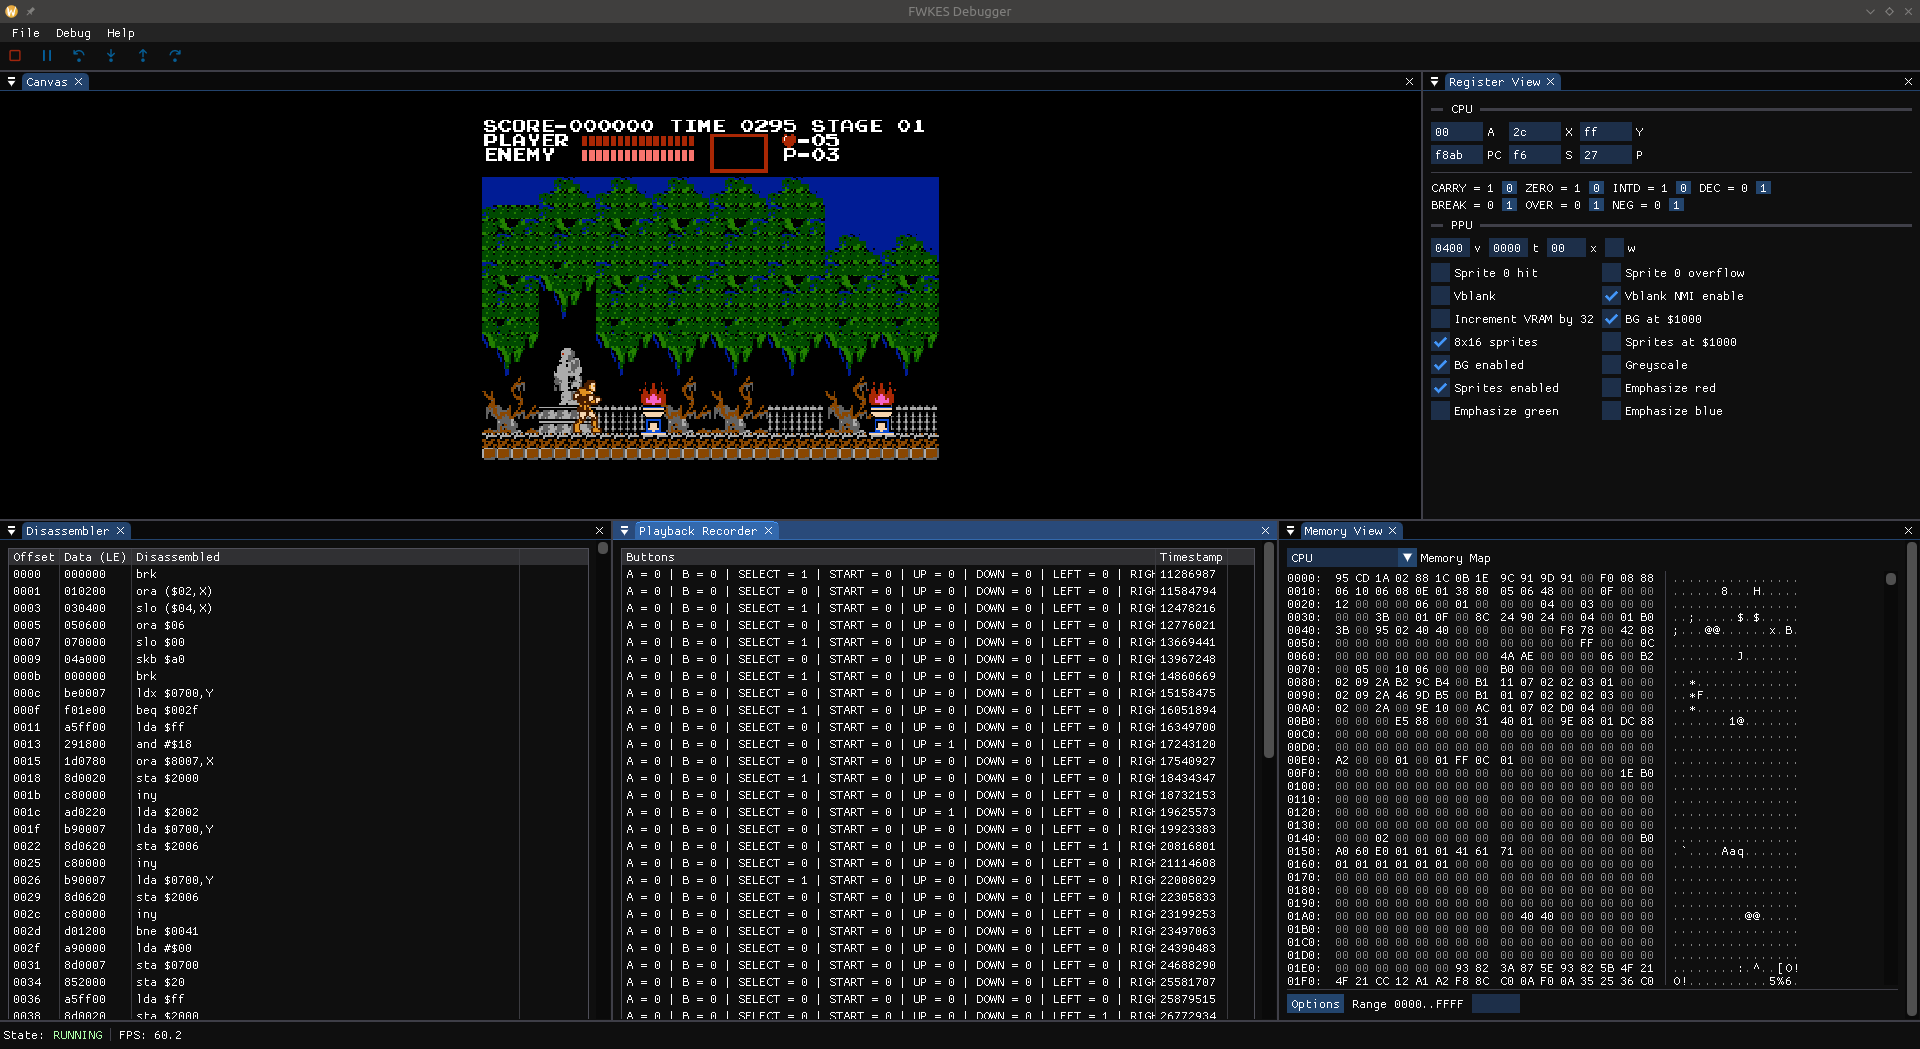
\includegraphics[width=\textwidth]{images/debugger.png}
    \caption{Screenshot debuggeru.}
    \label{fig:debugger}
\end{figure}

Do budoucna se plánuje pokročit dál a vyvinout plnohodnotné vývojové prostředí, které dovolí
nejen ladit NES programy, ale také i psát vlastní.

\section{Závěr}

Výsledný emulátor dosahuje vysoké míry věrnosti původnímu hardwaru, která v mnoha ohledech překonává
běžné amatérské implementace. Přestože z hlediska absolutní přesnosti
zatím nedosahuje úrovně dlouhodobě vyvíjených a vysoce precizních projektů, jako jsou
Mesen, FCEUX nebo Nintendulator, je schopen korektně a plynule spustit
drtivou většinu titulů využívajících podporované mappery (NROM, UNROM a MMC3). V těchto případech
obrazový i zvukový výstup věrně odpovídá chování originálního systému.

Drobné odchylky se projevují pouze ve velmi specifických scénářích, nejčastěji v podobě drobných
vizuálních artefaktů. Ty jsou důsledkem vědomého zjednodušení některých pokročilých vlastností PPU,
konkrétně absence podpory pro emphasis bity a základní implementace ořezu okrajů obrazu
(\textit{clipping}). Vzhledem k tomu, že tyto specifické funkce využívá pouze úzká skupina her,
zůstává celková hratelnost a uživatelský zážitek u naprosté většiny testovaných titulů neovlivněn.

% Výsledný emulátor vykazuje poměrně vysokou míru věrnosti původnímu hardwaru. Je schopen bezchybně spustit
% naprostou většinu her využívajících mappery NROM, UNROM a MMC3. Ve většině
% případů odpovídá obrazový i zvukový výstup originálnímu systému. Drobné odchylky se mohou projevit
% ve velmi specifických situacích, například ve formě vizuálních artefaktů, které jsou způsobeny
% neimplementovanými nebo zjednodušenými vlastnostmi hardwaru.

% Mezi známé omezení patří neimplementované \textit{emphasis} bity a zjednodušené řešení ořezu obrazu
% (clipping). Tyto vlastnosti mají vliv pouze na úzkou skupinu programů a ve většině případů
% neovlivňují hratelnost.
